\documentclass[12pt, block=fill]{beamer}
\usepackage{graphicx}
\usepackage[sfdefault]{FiraSans}
\usepackage{FiraMono}
\usepackage[T1]{fontenc}
\usepackage{xcolor}
\usepackage{mathtools}

\usepackage{hyperref}
\usepackage{tabularx}

\definecolor{burntOrange}{rgb}{.8, .5, .1}
\definecolor{textgray}{rgb}{.8,.8,.8}
\definecolor{berkeleyYellow}{HTML}{FDB515}

\usepackage{dcolumn}

\newcommand{\alex}[1]{\textcolor{berkeleyYellow}{#1}}
\newcommand{\paul}[1]{\textcolor{red}{#1}}

\usetheme[
titleformat frame = smallcaps,
subsectionpage = progressbar]
{metropolis}

\metroset{
  block=fill
}
\newcommand{\E}{\text{E}}
\newcommand{\V}{\text{V}}
\newcommand{\cov}{\text{cov}}

\newcommand{\Z}{\mathbb{Z}}
\newcommand{\R}{\mathbb{R}}
\newcommand{\N}{\mathbb{N}}
\newcommand{\indep}{\mathrel{\text{\scalebox{1.07}{$\perp\mkern-10mu\perp$}}}}

\newcommand{\bluecheck}{}%
\DeclareRobustCommand{\greencheck}{%
  \tikz\fill[scale=0.8, color=green]
  (0,.35) -- (.25,0) -- (1,.7) -- (.25,.15) -- cycle;%
}
\usepackage{pifont}
 \newcommand{\xmark}{\textcolor{red}{\ding{55}} }

\usepackage{pgfpages}
\setbeameroption{hide notes} % Only slides
% \setbeameroption{show only notes} % Only notes
  % \setbeameroption{show notes on second screen=right}
  % Both

\title{Week 10}
\subtitle{Questions of Description}

\author{Paul Laskowski and Alex Hughes}
\institute{UC Berkeley, School of Information}

\begin{document}

\begin{frame}
  \maketitle
\end{frame}

\section{Questions of Description}

\begin{frame}

  \note[item]{Here are some questions that you might want to answer
    with a statistical analysis...}
  \frametitle{Questions of Description}
    \includegraphics[width = \textwidth]{images/gdp}
    What is the shape of the relationship between a country's
    economic output and Internet access?
\end{frame}

\begin{frame}
  \frametitle{Questions of Description}
   \begin{center} \includegraphics[width = .5\textwidth]{images/equal_pay}
    
  \vspace{-.8cm} \footnotesize Image: Alarichall (CC SA 4.0)
   \end{center}
   
    How big is the pay gap in the United States? \note[item]{That is, what
      is the difference in pay between workers of different genders?}
\end{frame}

\begin{frame}
  \frametitle{Questions of Description}
    \includegraphics[width = \textwidth]{images/pay_age}
     How does the pay gap depend on the age of the worker?
\end{frame}

\begin{frame}[standout]
Description
  \note[item]{One thing these questions have in common: They are
    questions of description.}  \note[item]{They are also questions
    that can be addressed using linear regression.}
  \note[item]{You've learned the mechanics of how linear regression
    works.  You know the nuts and bolts of interpreting coefficients and statistical guarantees.}
    \note[item]{But how do you build a model, when the purpose is description.  that's a more strategic level of thinking}
    \note[item]{There's an entire set of concerns that goes into building models for description, and that's going to be out topic in this unit.}
    
\end{frame}



\begin{frame}
  \frametitle{Plan for the Week}
  
  Preamble
  \begin{itemize}
  \item Three modes of model building
  \end{itemize}
  
  Three sections about descriptive modeling
  \begin{enumerate}
  \item Capturing nonlinear relationships
  \item Measurement with controls
  \item Modeling conditional effects
  \end{enumerate}
\end{frame}

\begin{frame}
  \frametitle{Plan for the Week (cont.)}
  At the end of this week, you will be able to:
  \begin{itemize}
  \item Understand how three major modes of model building lead to
    very different models
  \item Balance design goals when creating a model for description
  \item Plan a set of model specifications for a regression table
  \end{itemize}
\end{frame}

\section{What Is Linear Model Building?}

\begin{frame}
  \frametitle{What Is Linear?}
  \centering \renewcommand{\arraystretch}{1.6}
  \begin{tabular}{r|c}
    Model & Linear?\\
    \hline
    $ Y= \beta_0 + \beta_1 X_1 + \beta_2 X_2 + \epsilon$ &\\
    $Y = \beta_0 + \beta_1 X + \beta_2 X^2 + \epsilon$  & \\
    $\ln Y = \beta_0 + \beta_1 \ln X + \epsilon$ & \\
    $Y = \beta_0 X ^ {\beta_1} + \epsilon $ &\\
  \end{tabular}
  \note[item]{Before we talk about model building, let's review a
    basic definition.  What makes a linear model linear?}
  \note[item]{Here's our classic linear model equation, you know this
    is linear, but why?}  \note[item]{You might answer, $Y$ is linear
    in the $X$'s.  But that's not quite right.  What's important here
    is Y is linear in the terms.}  \note[item]{Here's a model, where
    we've squared X.  If you think about it, this is the equation for
    a parabola, not a line.  But actually, you can run an ols
    regression on this, no problem, because $X$ and $X^2$ are just
    like two variables.}  \note[item]{Another example, where we've
    taken logs of Y and X.  That's no longer the equation for a line,
    but we've just created new variables, and we can run an ols
    regression on them.}  \note[item]{That's not to say that
    everything in the world is linear.  Here's an example of an
    equation that's not allowed in OLS} \note[item]{But I'm hinting at
    the fact that there's a lot more flexibility in the linear model
    than you might think at first.}
\end{frame}



\begin{frame}
  \frametitle{What Is Linear Model Building?}

  \note[item]{Once you recognize that there are actually a lot of
    different models that count as linear, you might wonder: how do
    you choose one?}
  
  How do you select from all the possible linear models?

  \note[item]{Here are some more specific questions that you face as a
    data scientist}
  
  \begin{itemize}
  \item Which variables to include, which to exclude
  \item Whether and how to transform each variable
  \item Whether to create new variables
  \item Whether to multiply variables together
  \end{itemize}
  
\end{frame}


\begin{frame}
  \frametitle{The Model-Building Process}
  \note[item]{Here's a very very rough schematic, just to emphasize
    that model building is usually an iteratie prcess. You propose a
    model, then evaluate it, then make adjustments and propose a new
    model} \note[item]{When you are proposing a model, here are some
    of the factors that will guide your decision} \note[item]{And when
    you are evaluating}
  
  \includegraphics[width = \textwidth]{images/propose_evaluate}
  
  \begin{columns}
    \begin{column}{0.5\textwidth}
      \begin{itemize}
      \item Modeling goals
      \item Observations from data
      \item Background knowledge
      \item Background theory
      \end{itemize}

    \end{column}
    \begin{column}{0.5\textwidth}
      \begin{center}
        \begin{itemize}
        \item Diagnostic plots
        \item Measures of fit
        \item Tests of model assumptions
        \end{itemize}
      \end{center}
    \end{column}
  \end{columns}
  \note[item]{In the following segments, we're going to dig into all
    of these components, and give you an idea of wha this process is
    like}
\end{frame}

\section{Modes of Model Building}


\begin{frame}[standout]
  \frametitle{An Important Question to Keep in Mind:}
  What are your goals?  \note[item]{If I can give you one piece of
    advice as you start model building, it's to keep this question in
    your mind: what are your goals?}  \note[item]{\paul{scribble in
      "modeling"}} \note[item]{Depending on what your modeling goals
    are, even if you have the same data, you may end up with very very
    different models.}  \note[item]{That's true of linear regression
    specifically.  A statistician, a political scientist, and a
    machine learning researcher can all use linear regression on the
    same data, but the models will look very differerent.  Those
    differences can be traced to the different goals that each of
    those people have.}
\end{frame}


\begin{frame}
  \frametitle{Three Modes of Model Building}
  \note[item]{So there is a large variety in the way that people in
    different fields build models.}  \note[item]{At the same time, we
    can identify three major modes of model building that account for
    most of the variety we see: predictive, descriptive, and
    explanatory.  It's important that you understand the differences
    between them, and the goals that are common in each one.}

  \begin{enumerate}
  \item Predictive modeling: What value can we expect for data we
    haven't seen?
  \item Descriptive modeling: How can we make sense of the patterns
    in data?
  \item Explanatory modeling: How can we measure effects inside a
    causal theory?
  \end{enumerate}

\end{frame}

\subsection{Predictive Modeling}

\begin{frame}
  \frametitle{Predictive Modeling}
  
  \note[item]{Let's start with predictive modeling.  When we say
    prediction, we mean computing a guess for data we haven't seen.}
  \note[item]{It could be new people.  Ex: you get data about a
    patient's symptoms and you want to predict if they have an immune
    disorder.}  \note[item]{It could also be future values.  Ex. given
    the last 3 years of data, how many waffle irons can we sell next
    december?}
  
  \textbf{Prediction:} making guesses for unknown values
  \begin{itemize}
  \item For new people, new pictures of cats, or other units
  \item For future time periods
  \end{itemize}
  
  \note[item]{When we think about predictive modeling, the field that
    immediately jumps to mind is machine learning, especially
    supervised machine learning.  But a lot of time series analysis is
    also very focused on prediction.}

  A key focus of machine learning and time series analysis
\end{frame}

\begin{frame}
  \frametitle{Key Goals of Predictive Modeling}
  \begin{enumerate}
  \item Accurately predict values \note[item]{What are the goals of
      predictive modeling?  Number 1: accuracy - make predictions that
      are as close to ground truth as possible.}  \note[item]{In a
      way, predictive modeling is the most well-defined mode of model
      building, because it usually has just this one goal.  The
      internals of the model don't matter as long as it predicts well.
      So you have a lot of flexibility when it comes to choosing the
      model, you can try a neural network, then switch to a random
      forest.  still, linear regression is still important here.}
    
    \note[item]{It is true that sometimes there is a second goal in
      predictive modeling, being interpretable. }  \note[item]{This is
      especially true when a model makes decisions for humans, such as
      who gets a loan and who doesn't.  But those situations are less
      common - most of the time, interpretability doesn't matter very
      much.}
  \item Be interpretable by humans (usually less important)
    
  \end{enumerate}
  
  Implications for linear regression
  \begin{itemize}
  \item Hundreds of variables, or more  \note[item]{When we care
      about prediction, why not try every possible variable we can get
      our hands on?}
  \item Variable selection by algorithm \note[item]{Because we have so
      many variables, we'll need algorithms to select the ones that
      make it to the final model. }
    \begin{itemize}
    \item False discovery: Out of many variables, some will look
      important by chance.  \note[item]{In ML this is called
        overfitting.  There is a long list of specialized techniques
        to combat this.}
    \end{itemize}
  \item Coefficients usually don't have meaning \note[item]{As a
      result of these features, individual coefficients usually don't
      have any meaning.  They may change completely in response to
      tiny perturbations in the data}
  \end{itemize}
\end{frame}

\subsection{Descriptive Modeling}

\begin{frame}
  \frametitle{Descriptive Modeling}
  \textbf{Description:} summarizing or representing data in a compact,
  human-understandable way
 
  \begin{itemize}
  \item Gain understanding by interpreting the model's internal
    structure
  \item Popular in statistics, but ``not commonly used for theory
    building
    and testing in other disciplines''\\
    \hspace{1cm}—Shmueli, Galit.\textit{ To Explain or to Predict?}
  \end{itemize}

  \note[item]{Descriptive modeling is really popular among
    statisticians, but not very popular outside of statistics.  Why?
    Associations are not Causations}
\end{frame}

\begin{frame}
  \frametitle{Key Goals of Descriptive Modeling}
  
  \begin{enumerate}
  \item Measure complex concepts \note[item]{We want to measure
      complex concepts, or especially relationships}
  \item Capture features of the world \note[item]{We want to capture
      features of the world.  This overlaps with making accurate
      predictions, but it's not really the same goal.  we want to
      capture features that help us make sense of the world.}
  \item Simplify phenomena to make them understandable
  \item Highlight associations
  \item Generate hypotheses
  \end{enumerate}
  
  Implications for linear regression
  \begin{itemize}
  \item Parsimonious models
  \item Use of logarithms and other transforms with clear
    interpretation
  \item Long build process relying on EDA
  \end{itemize}
\end{frame}

\subsection{Explanatory Modeling}

\begin{frame}
  \frametitle{Explanatory Modeling}
  \textbf{Explanation:} using data to test or estimate parameters in a
  causal theory
 
  \note[item]{Why is this important?  Because we may want to learn
    something from a model and then DO something.  Maybe we want to
    set a policy to improve public health.  Maybe we want to change
    our prices to increase profits. }  \note[item]{Business problems
    are also usually causal.  You want to know what will happen if the
    business changes its prices, or adopts a new policy.  You don't
    care if lower prices are associated with more profit, you want to
    know what will happen if you actually change the prices. }
 
  \note[item]{I want to point out something in our definition - the
    causal theory is there first, then we combine it with data.  It
    may not be a big Theory with a capital T.  However: You always
    need to start with some causal background information.  We'll come
    back to this point in our unit on explanatory modeling.}
  

  \begin{itemize}
  \item Explanation lets us reason about actions
  \item Common mode in economics, political science, epidemiology,
    psychology, environmental science...
  \item Causal assumptions are required to make causal claims

  \end{itemize}
 
\end{frame}


\begin{frame}
  \frametitle{Key Goals of Explanatory Modeling}
  \begin{enumerate}
    \note[item]{very often, our primary goal is measuring a causal
      effect.  that's asking, if we manipulate one variable $X$, what
      will be the resulting effect on $Y$.  We want to know the
      strength of that relationship.}
  \item Measure a causal effect.
  \item Evaluate a theory.
  \item Predict the consequences of potential actions.
  \end{enumerate}
  
  Implications for linear regression
  \begin{itemize}
  \item Variable selection is guided by causal theory
  \item Models oriented to perform a specific measurement
  \item Key challenge is the operationalization gap between
    theoretical constructs and variables
  \end{itemize}
\end{frame}


\begin{frame}
  \frametitle{Three Modes of Model Building}

  \note[item]{So there you have the three major modes of model
    building.  We've seen that each of them has very different goals,
    which leads to quite different linear models.  Let me also point
    out that the divisions aren't always that clear.  In descriptive
    modeling, a key goal is capturing features of the joint
    distribution.  But of course, that can also help us to make sense
    of an explanatory model.  In fact, trying to capture features of
    the joint distribution can sometimes lead you to more accurate
    machine learning models for prediction.  }  \note[item]{But as you
    keep learning, it can really help to pay attention to which of the
    three main modeling modes you're working in..}
  \begin{enumerate}
  \item Predictive modeling: What value can we expect for data we
    haven't seen?
  \item Descriptive modeling: How can we make sense of the patterns
    in data?
  \item Explanatory modeling: How can we measure effects inside a
    causal theory?
  \end{enumerate}

\end{frame}


\section{Introduction to Descriptive Modeling}

\begin{frame}
  \frametitle{How Would You Describe These Data?}
  \centering \includegraphics[width = \textwidth]{images/cars}
  \note[item]{If you had to describe this data over the phone, how
    would you do it?  Take 10 seconds, and try to say a few words
    about it right now.}  \note[item]{What words are you using?
    Slope? Decreasing? Maybe hyperbolic or exponential?}
  \note[item]{If you used any of those words, really, what you're
    doing right now is descriptive model building} \note[item]{You may
    be doing it very informally, or even subconsciously, but you're
    probably imagining a smooth curve passing through these points and
    describing that curve.}
\end{frame}


\begin{frame}
  \frametitle{Introduction to Descriptive Modeling}

  \note[item]{ Let's review what Description means.}
  \textbf{Description:} summarizing or representing data in a compact,
  human-understandable way
 
  \note[item]{There are many tools we can use for describing data.
    There's clustering algorithms, principle component analysis, and
    linear regression is also a description tool}
 
  Linear regression is a tool that can help us answer:

  \begin{itemize}
  \item What patterns exist in a dataset?
  \item What is the shape of a specific relationship?
  \item What is the size of a feature or effect?  \note[item]{the
      sizes of different features are encoded in the coefficients!}
    \note[item]{Unlike a predictive model, in a descriptive model, we
      really care about our betas, they are measurements of the
      world.}
  \end{itemize}

\end{frame}




\begin{frame}
  \frametitle{What Does It Take to Build a Descriptive Model?}

  Skill, art, and a lot of iteration

  \begin{itemize}
  \item No causal theory to constrain model choice
  \item Often many ways to operationalize concepts
  \item Need to balance many competing goals
  \item Takes time to build intuition in many dimensions
  \end{itemize}

  \note[item]{All together this can be a very creative form of model
    building.}  \note[item]{It's our main topic for today - I hope
    you're excited to dive in.}

\end{frame}



\section{Logarithms}

\begin{frame}
  \frametitle{A Question of Development}
  
  How does the economic productivity of a country relate to Internet
  access?
  
  Data taken from the World Bank
  \begin{itemize}
  \item GDP per capita
  \item Internet users per 100
  \end{itemize}

  
\end{frame}



\begin{frame}
  \frametitle{Is OLS Regression Appropriate?}

  \includegraphics[width = \textwidth]{images/gdp1}

  \note[item]{Here's a graph of our data.}
  \note[item]{You can see it
    has this very interesting pattern - a very nonlinear pattern.  Try
    taking your finger, and drawing a line to represent this data.
    Take a moment to think about this question: is it ok to run a
    linear regression?  here?}
  \note[item]{\paul{Alex: turn this into
      a learnosity check?}}
  \note[item]{The short answer is that you
    can absolutely run an ols regression.  We know that OLS
    coefficients are consistent for the best linear predictor, as long
    as the best linear predictor exists and is unique.  (there is
    another assumption to worry about, which is iid.  Can you really
    believe that countries are independent from each other? I'm
    skeptical, but there are a lot of country-by-country studies out
    there, so let's note the problem as a limitation but keep going.)}
\end{frame}


\begin{frame}
  \frametitle{Interpreting the Level-Level Model}
  
  \note[item]{Here's are the results of fitting the ols regression}
  
  $$\widehat{users} = 2.4 + .0021\ GDP$$
  
  \note[item]{Here's how we would interpret the coefficient...}
  
  \textbf{Interpretation 1:} A country with an extra \$1 of GDP per
  capita is predicted to have another .0021 Internet users per 100.
  \note[item]{Both of these numbers are really small.  So we can
    improve this interpretation by choosing a bigger change...}

  \textbf{Interpretation 2:} A country with an extra \$1,000 of GDP
  per capita is predicted to have another 2.1 Internet users per 100.
\end{frame}

\begin{frame}
  \frametitle{Does OLS Regression Meet Our Goals?}
  \includegraphics[width = \textwidth]{images/gdp2}
  \note[item]{Here's what the regression line looks like.  We know
    this is valid as far as ols assumptions.} 
  \note[item]{But does it meet our goals?  In particular, one of the
    main goals of descriptive modeling is capturing features of the
    world.} 
  \note[item]{There's a clear structure that is not reflected in our
    model.}  \note[item]{If you look in the middle section, you can
    see that the prediction is consistently too low.  At the extremes,
    the prediction is too high.}
  \note[item]{There's one other small problem that's worth mentioning.
    it's only a minor problem, but notice that most of the data is
    clustered on the left side.  The slope of the line is mostly
    determined by these few points on the right side.  that's ok, but
    there's these points on the left potentially have important
    information that's not really making it into the model.}
  \note[item]{For all these reasons, we need to consider a variable
    transformation.}
\end{frame}

\begin{frame}
  \frametitle{Variable Transformation}

  \note[item]{Transforming a variable, means that we're replacing some
    X with a function f(X)}

  \begin{block}{\textbf{Variable transformation}}
    Replace $X$ with $f(X)$ for some $f: \R \rightarrow \R$
    \note[item]{What function $f$ should you use?  Here are some of
      the most common choices.}
    \begin{itemize}
    \item $\ln(X)$
    \item $\log_{10}(X)$
    \item Indicator functions
    \item $X^a$
    \item Polynomials(X)
    \end{itemize}
    \note[item]{Out of all of these, the logarithm is the probably the
      best choice for our data.  Let's see what it does.}
  \end{block}
\end{frame}


\begin{frame}
  \frametitle{Taking the Log of GDP}

  \includegraphics[width = \textwidth]{images/gdp3} \note[item]{Here's
    what the data looks like after you take a log of GDP per capita.
    Can you draw a line through it?  Much easier!}
\end{frame}

\begin{frame}
  \frametitle{Taking the Log of GDP}

  \includegraphics[width = \textwidth]{images/gdp4} \note[item]{And
    here is the new regression line, which matches the shape of this
    relationship.}
\end{frame}


\begin{frame}
  \frametitle{Model: $\widehat{users} = \beta_0 + \beta_1 \ln GDP \quad\quad R^2 = .68$}

  \centering
  \includegraphics[width=\textwidth]{images/gdp5}

  \note[item]{There's another way to view this model.  Let's go back
    to the original x-axis, without the log} \note[item]{If we do
    that, this is what our model looks like} \note[item]{This is a
    logarithmic curve.  That makes sense.  Our model says that
    predicted internet users is a linear function of the log of GDP.}
  \note[item]{Think about it this way, we took the log of X and
    revealed a straight line in the scatterplot.  That tells us that
    we have a logarithmic relationship.}  
\end{frame}

\section{Interpreting and Applying Logarithms}

\begin{frame}
  \frametitle{Interpreting Logarithms}
  \note[item]{There are actually two common choices for the logarithm,
    you can take a base 10 log, or a natural log} \textbf{Base 10 log}
  \note[item]{A base 10 log is helpful when we want to think about a
    variable in powers of 10.  We're all used to powers of 10.}
  $$\widehat{users} = -66.5 + 32.0 \log_{10} GDP$$
  Interpretation: adding a 0 to GDP associated with 32 more Internet
  users per 100
  
  \textbf{Base $e$ log}
  
  $$\widehat{users} = -66.5 + 13.9 \ln GDP$$
  
  Interpretation: multiplying GDP by a small $1+\alpha$ associated with
  $13.9 \alpha$ more Internet users per 100
\end{frame}

\begin{frame}[t]
  \frametitle{Interpreting Logarithms (cont.)}
\note[item]{  $\frac{\partial}{\partial x}\ln x = 1/x$ }
$$ \frac{\partial \widehat{users}}{\partial GDP} =
                                                    \frac{\partial}{\partial GDP} [ -66.5 + 13.9\ln GDP ] $$
\note[item]{\begingroup
  \addtolength{\jot}{1em}
  \begin{align*}
                                                  &= 13.9 \frac{1}{GDP} \\
    \partial \widehat{users} &= 13.9 \frac{\partial GDP}{GDP} \\
 \Delta \widehat{users}  &\approx 13.9 \frac{\Delta GDP}{GDP}
  \end{align*}
  \endgroup}
  
\end{frame}

\begin{frame}
  \frametitle{Model:
    $\widehat{users} = \beta_0 + \beta_1 \ln GDP \quad\quad R^2 = .68$
  }
  \includegraphics[width = \textwidth]{images/gdp5}
  \note[item]{Let's see what that rule of thumb looks like on the
    graph. Let's choose some point on the curve, GDP = 10,000.}
  \note[item]{I'm going to draw the tangent line at that point - it's
    a good approximation for small changes in GDP.}
  \note[item]{I know the slope of the tangent is 13.9/GDP}
  \note[item]{Let's say that I increase GDP by some proportion,
    $\alpha GDP$ so I can mark that as the change in X.}
  \note[item]{What's the change in Y?  I multiple the change in
    X by the slope and I get $13.9 \alpha$}
  \note[item]{If alpha is small, then the tangent line is close to the
    curve, so this is a good approximation.} 
  \note[item]{For example, if we increase GDP by 1\%. Then
    $\alpha=.01$ then we'll get .139 more users.} 
  \note[item]{But if you think about really big changes: 30\% or 50\% 
    increases, the approximation gets worse and worse.}
\end{frame}


\begin{frame}
  \frametitle{Other Uses of Logarithms}

  Log-linear form: $\ln Y = \beta_0 + \beta_1 X$
  \begin{itemize}
  \item Interpretation: $\frac{\Delta Y}{Y} \approx \beta_1 \Delta X$
  \item Example: add 0.1 to $X$ $\rightarrow$ add $0.1 \beta_1 \cdot Y$ to
    $Y$
  \end{itemize}

  Log-log form: $\ln Y = \beta_0 + \beta_1 \ln X$
   
  \begin{itemize}
  \item Constant elasticity model
  \item Interpretation:
    $\frac{\Delta Y}{Y} \approx \beta_1 \frac{\Delta X}{X}$
  \item Example: increase $X$ by 1\% $\rightarrow$ increase $Y$ by
    $\beta_1 \%$
  \end{itemize}
\end{frame}

\begin{frame}
  \frametitle{When to Apply Logs}
  What makes a variable a good candidate for a log transform?
  \begin{itemize}
  \item Always positive
    \begin{itemize}
    \item Don't add a constant to make variable positive
    \end{itemize}
  \item Spans multiple orders of magnitude
  \item Clustered near zero with high outliers
  \item Percent changes are meaningful \note[item]{This is especially 
      true for monetary variable.  We all understand what a 20\%
      increase in salary is.  A dollar increase can feel very
      different depending on how much money you have, but 10\% more is 
      meaningful for almost everyone.  }
  \end{itemize}
\end{frame}

\begin{frame}
  \frametitle{Power Transformations}
  
  \note[item]{\paul{Alex, tried to trim this down, but also happy to
      skip the slide.}}
  \note[item]{I want to very quickly mention a broader class of
    transformations, called the power transformations}
  \note[item]{Here, we're raising X to a power.}
  \note[item]{For example, you might take the square root of X in
    situations where you can't take the log, because a variable
    sometimes equals zero.}
  \note[item]{However, these transformations make it much harder to
    interpret the results of a model, so they're not used very often
    in descriptive modeling.} 
  \textbf{Power transformation:} Replace $X$ with $X^\alpha$ for some
  $\alpha \in \R$.
  \begin{itemize}
  \item $\sqrt{X}$ behaves similarly to $\ln X$.
  \item $X^2$, $X^3$,... spreads values far from zero further apart.
  \end{itemize}
  Interpretation is more difficult than with logs.
\end{frame}

\begin{frame}
  \frametitle{When to Apply Transformations}

  \textbf{Question:} Should you always transform your variables to
  make them normal?  \note[item]{Before we move on, I want to address
    one issue, a lot of websites will tell you to always transform
    your variables until they look normal.  Is that a good idea?}
  \begin{itemize}
  \item Normal variables are \textbf{never} a requirement for OLS
    regression.
    \begin{itemize}
    \item Even in the classical linear model, \textit{errors} are
      normal, not variables.
    \end{itemize}
  \end{itemize}
  $\implies$ Don't focus too much on normality.  Capturing relationships
  is more important.  \note[item]{Well, first of all, normal variables
    are never a requirement for ols. Even in the classical linear model,
    the errors must be normal, not the variables.  Of course if you're
    in a large sample, there's no assumption of normality at all.}
  \note[item]{ But I will say that normal variables are generally a good
    thing.  Normal means that most of your data isn't so clustered that
    it doesn't affect the model.  So it's good to try for normal
    variables, but bad if that's the only thing you're thinking about}
  \note[item]{Remember, your goals for descriptive modeling.  In
    particular, transforms are great for the goal of capturing features
    of the world.  that means looking at scatterplots, and trying to
    reveal linear patterns.  If you can make your scatterplots look
    linear, that's usually much more important than having nice normal
    distributions.}
\end{frame}

\section{Polynomials}

\begin{frame}
  \frametitle{How Can We Improve Predictive Accuracy?}
  \includegraphics[width = \textwidth]{images/gdp1}
  
  \note[item]{Here's another look at our GDP and Internet User data.
    Previously, we used a log transform.  That was good for capturing
    the shape and great for model interpretability.}
  \note[item]{What if I tell you that your goals are little different.  You still
    care about interpretation, but you really want more accuracy.
    You'd be willing to give up a little bit of interpretability to
    get a higher $R^2$}
  \note[item]{In that case, you might want to consider a polynomial regression.}
\end{frame}


\begin{frame}
  \frametitle{Polynomial Regression}
  
  \note[item]{First, why polynomials?  well, polynomials are really
    flexible.  They can approximate any continuous function.  }
  Motivation: Polynomials can approximate any continuous function
  (e.g. Weierstrass theorem)
  
  \vspace{.5cm} \note[item]{The idea here is we're going to run a
    regression with different powers of the same variable.}
    
  \note[item]{Most of the time, we'll use just a quadratic.  So we'll
    put in GDP and $GDP^2$} Quadratic:
  $\widehat{Users} = \beta_0 + \beta_1 GDP + \beta_2 GDP^2$
 
  \note[item]{What will ols regression do?  ols finds the beta's that
    minimize MSE.  If you change these betas, you get all the
    different parabolas in the X-Y plane.}
  \begin{itemize}
  \item OLS finds the parabola that minimizes MSE.
  \end{itemize}
  
  \note[item]{You can also put in the cubic term, though that's much
    less common.}
  
  Cubic:
  $\widehat{Users} = \beta_0 + \beta_1 GDP + \beta_2 GDP^2 + \beta_3 
  GDP^3$ 
 \begin{itemize}
  \item OLS finds the cubic function that minimizes MSE.
  \end{itemize}
\end{frame}

\begin{frame}
  \frametitle{A Parabolic Pattern?}
  \note[item]{Let's try the quadratic form.}
  \includegraphics[width=\textwidth]{images/gdp1}
  \note[item]{Here's the data again.  I want you to imagine what you
    think the best fitting parabola looks like.  try tracing it with
    your finger.}
\end{frame}


\begin{frame}
  \frametitle{Model:
    $\widehat{users} = \beta_0 + \beta_1 GDP + \beta_2 GDP^2
    \quad\quad R^2 = .66$ }

  \note[item]{There you have the best fitting parabola}
  \includegraphics[width = \textwidth]{images/gdp6} \note[item]{You
    can see that it definitely looks closer to the data than the line.
    The fit is actually slightly worse }
\end{frame}


\begin{frame}
  \frametitle{Interpreting the Quadratic Specification}
  
  $$\widehat{Users} = 18.5 + .0048\ GDP - 8.0\cdot 10^{-8}\ GDP^2$$
  
  \note[item]{Here's the equation with the fitted coefficients}
  \note[item]{What's the interpretation of this equation?}
  \note[item]{Let's look at the slope... we get a function - the partial
    depends on GDP}
  
  $$\frac{\partial \widehat{Users}}{\partial GDP} = .0048  - 1.6\cdot 10^{-7}\ GDP$$
  
  Example 1: If $GDP = 10,000$, then
  $\frac{\partial \widehat{Users}}{\partial GDP} = .0032$.
  
  (Extra \$1,000 in GDP associated with 3.2 extra users)
  
  Example 2: If $GDP = 20,000$, then
  $\frac{\partial \widehat{Users}}{\partial GDP} = .0016$.
  
  (Extra \$1,000 in GDP associated with 1.6 extra users)
  
\end{frame}


\begin{frame}
  \frametitle{Higher-Order Polynomials}
  \includegraphics[width = \textwidth]{images/gdp9} \note[item]{what
    happens if we increase the order of our polynomial?}
  \note[item]{Here you can see the best fitting cubic function.
    Notice that the $R^2$ went up a bit - of course, we knew that
    would happen.  $R^2$ can only go up from adding variables.}
  \note[item]{The curve looks a little better at the end, it doesn't
    turn downwards.}  \note[item]{How far can we push this?  can we
    keep increasing the order of the polynomial and keep getting
    better and better predictions?}
\end{frame}


\begin{frame}
  \frametitle{Higher-Order Polynomials}
  \includegraphics[width = \textwidth]{images/gdp10}
  
  \note[item]{Here, I tried to fit an order 30 polynomial.  Indeed,
    the $R^2$ goes up even more.}
  \note[item]{But the shape doesn't make sense.  Why would internet
    users go up and down with GDP?}
  \note[item]{Especially on the right hand side, you can see that the
    curve traces from one point to the next.}
  \note[item]{This is a situation called overfitting.  We have a high
    $R^2$, but we're really just modeling the noise in this one
    dataset.  If we tried to use this model to predict internet users
    for a new set of countries, it would probably perform worse than
    the quadratic and cubic models.}
\end{frame}

\section{Measurement With Controls}

\begin{frame}
  \frametitle{Measurement With Controls}
  \textbf{Note:} This is a placeholder slide for an introduction that
  we will provide to the section. We're just placing it here for
  organization.
\end{frame}

\section{Interpreting Indicator Variables}


\begin{frame}
  \frametitle{Example: Measuring the Wage Gap}
  

  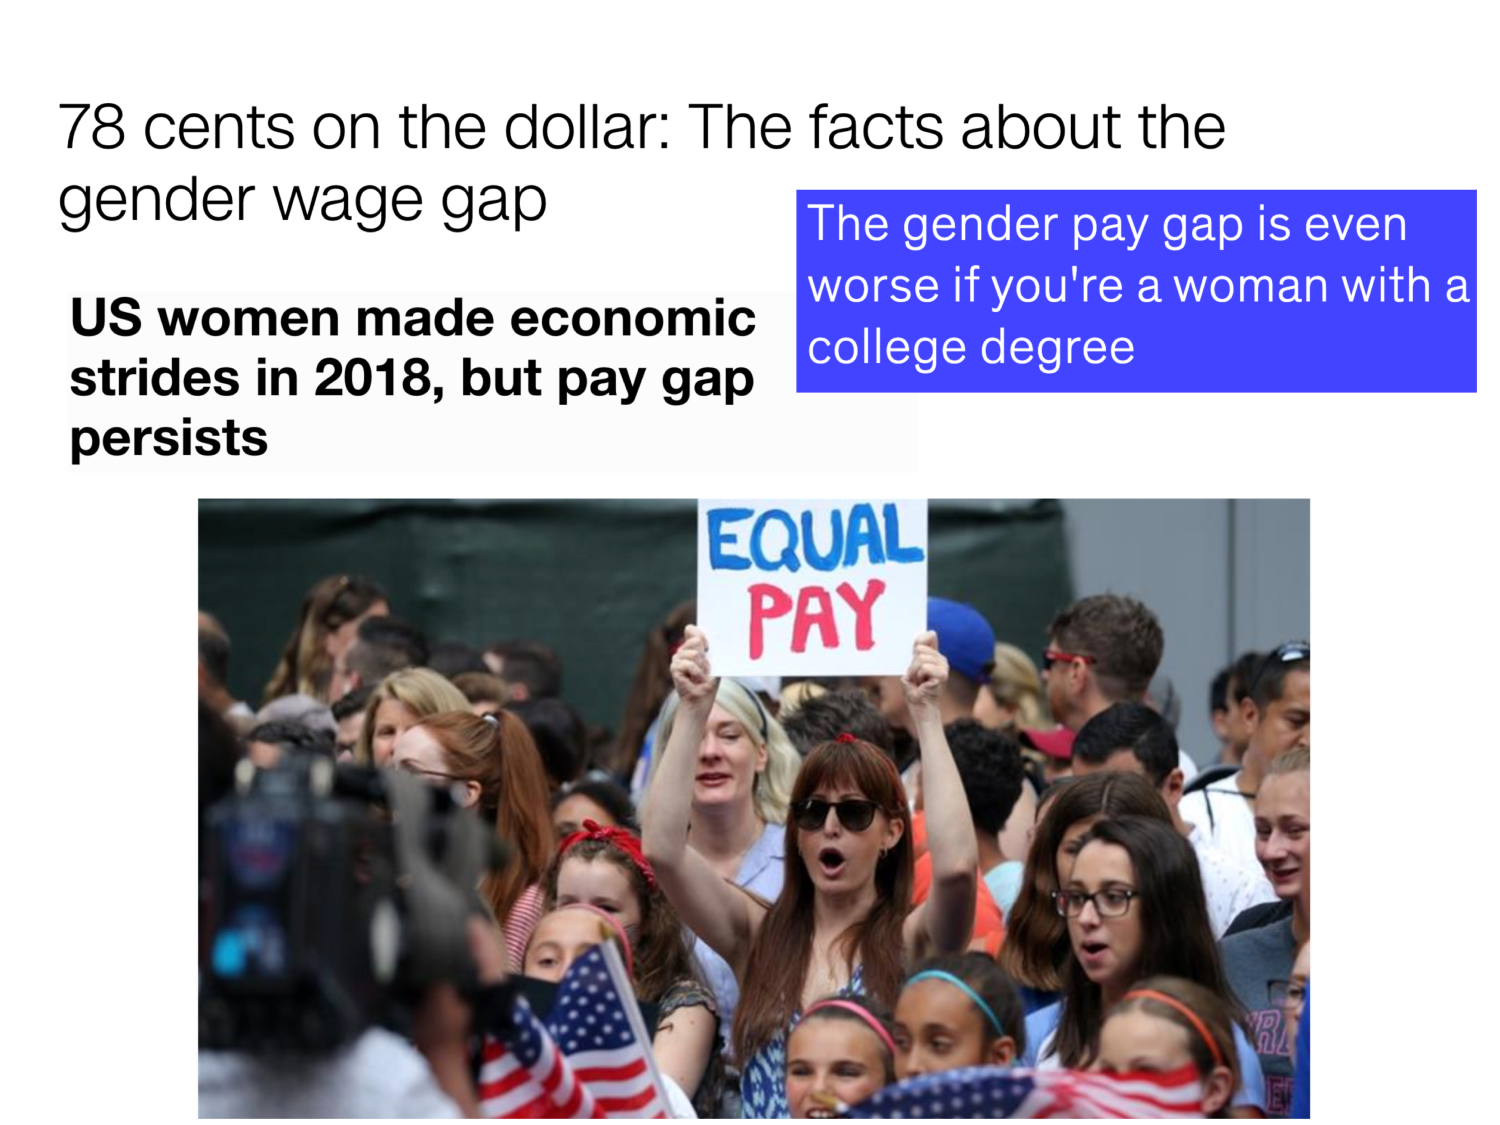
\includegraphics[width = \textwidth]{images/news}
 
  \note[item]{Let's take a look at an example measurement goal.  The
    example we'll use is the wage gap.}
  \note[item]{You probably already know about the wage gap -
    newspapers in the US talk about it from time to time.}
  \note[item]{In particular, you may have heard this figure: that a
    woman in the US earns 78 cents for every dollar that a man earns} 
  \note[item]{I hope you agree that this is an important topic - we
    would like to live in a country where people of all genders are
    paid equally} 
  \note[item]{But how can you actually measure the wage gap?  Should
    we compare all men and all women?  Or men and women in the same
    job?  But is that a fair comparison if people of different genders
    don't get the same job opportunities?  There's really no easy
    answer to these questions. But let's at least try measuring the
    gender gap and see what linear regression techniques may help.}
\end{frame}

\begin{frame}
  \frametitle{Example: Measuring the Wage Gap (cont.)}
  
  Data: Current Population Survey, 2019 Annual Social and Economic
  Supplement (ASEC)
  
  Key variables:
  \note[item]{In the survey, there is an income
    variable, and unlike most surveys, it's not binned into ranges,
    it's any integer.}
  \note[item]{The survey has no variable for
    gender, and it has one variable labeled sex.  You can see It only
    has two levels, male and female.  This is not a best practice,
    because it means that transgender and non-binary people may feel
    like they don't have an option.  Unfortunately, I have to say that
    we're filming this in 2020, and this is still what most big
    surveys are like. }

  \begin{itemize}
  \item Status: full-/part-time work status
    \begin{itemize}
    \item 1: not in labor force
    \item 2: full-time hours (35 or more), usually full-time\\
      \hspace{2cm} \vdots
    \end{itemize}

  \item Pay: total wage and salary earnings
  \item Sex
    \begin{itemize}
    \item 1: male
    \item 2: female
    \end{itemize}

  \end{itemize}
\end{frame}



\begin{frame}
  \frametitle{Overall Comparison}
  \note[item]{First, let's try the simplest thing we can do: comparing
    all men against all women.}
  
  \note[item]{Actually, we've seen this problem before.  When we
    talked about t-tests, we had two groups, and we wanted to know if
    the means were the same.}
  
  \includegraphics[width = \textwidth]{images/wage_hist}
  
\end{frame}


\begin{frame}
  \frametitle{Direct Application of t-Test}
  
  \note[item]{Here are the results of that t-test analysis.}
  \note[item]{You can see man pay for men about 69K, 52K for women,}
  \note[item]{That corresponds to about 76 cents to the dollar}
  \note[item]{The t statistic is giant - almost 30, so the null is
    overwhelmingly rejected} Mean for men: \$68,700
  
  Mean for women: \$52,100
  
  Mean difference: \$16,600
  
  (76 cents to the dollar)
  
  $t = 27.938, df = 61,733, p< 2.2e-16$

  \note[item]{Now, what about linear regression?  Well, it's important
    to realize that this exact analysis can be done in a regression
    framework.}
\end{frame}


\begin{frame}
  \frametitle{The Same Analysis in a Regression Framework, Part I}
  
  $$\widehat{Pay} = \beta_0 + \beta_1 Female$$
  
  For men, $\widehat{Pay} = \beta_0 + \beta_1 (0) = \beta_0$.
  
  For women,
  $\widehat{Pay} = \beta_0 + \beta_1 (1) = \beta_0 + \beta_1$.
  
  $\implies \beta_1$ represents the difference between groups.
  
  \note[item]{This may seem like a strange view of regression - aren't
    we supposed to be fitting a line?}
\end{frame}



\begin{frame}
  \frametitle{The Same Analysis in a Regression Framework, Part II}
  
  \begin{columns}
    \begin{column}{0.6\textwidth}
      \vspace{1cm} \includegraphics[width =
      \textwidth]{images/wage_slope}
    \end{column}
    \begin{column}{ 0.4\textwidth}
      $\Delta Y = \frac{\text{slope}}{\Delta X}$
    \end{column}
  \end{columns}


  \note[item]{Well, there is a line.  Here's what the data looks like
    if we plot it, and here's the regression line.  } \note[item]{(I
    took a small subset and added a little jitter so you can see
    things better.)}  \note[item]{Since we have an indicator variable,
    the only x values are 0 and 1 } \note[item]{What's the difference
    in in the predicted Y?...}  \note[item]{I can write:
    $\Delta Y = \frac{\text{slope}}{\Delta X} = \frac{\beta_1}{1} =
    \beta_1$}
\end{frame}


\begin{frame}
  \frametitle{The Same Analysis in a Regression Framework, Part III}
 \centering 
% Table created by stargazer v.5.2.2 by Marek Hlavac, Harvard University. E-mail: hlavac at fas.harvard.edu
% Date and time: Sat, May 23, 2020 - 08:51:38
\begin{tabular}{@{\extracolsep{5pt}}lc} 
\\[-1.8ex]\hline 
\hline \\[-1.8ex] 
 & \multicolumn{1}{c}{Dependent Variable: Pay} \\ 
\cline{2-2} 
\hline \\[-1.8ex] 
 Female & $-$16,561$^{***}$ \\ 
  & (618) \\ 
  & \\ 
 Intercept & 68,667$^{***}$ \\ 
  & (408) \\ 
  & \\ 
\hline \\[-1.8ex] 
Observations & 62,110 \\ 
\hline 
\hline \\[-1.8ex] 
\textit{Note:}  & \multicolumn{1}{r}{$^{*}$p$<$0.05; $^{**}$p$<$0.01; $^{***}$p$<$0.001} \\ 
\end{tabular} 


  \note[item]{When we look at our regression output, the coefficient
    for Female will have exactly the same difference in means that we
    say earlier.}  \note[item]{One more thing to note: we usually show
    a standard t-test for each coefficient.  Here, we have 3 stars for
    Female. The null of that test is that the slope is zero, which we
    know means that men and women are the same.  So this is exactly
    the same as the classic t-test for two groups.}
  \note[item]{Here's another question to think about: what do the
    stars on the intercept mean?}  \note[item]{Remember that the
    intercept represents the mean pay for men.  This is the test to
    see if men earn 0 dollars.  So that's a very silly test to run.
    But we do put in the stars anyway, just to be consistent.}
  \note[item]{How do you know if Women earn zero dollars?  We don't
    have that test here.  we'd have to run a separate command to get
    that test.}
\end{frame}



\section{Indicator Variables as Controls}

\begin{frame}
  \frametitle{Controlling for Occupation, Part I}
  \center How can we compare men and women in the same occupation?
  \note[item]{So far, we've just been comparing men as a whole to
    women as a whole} \note[item]{But part of the difference we see
    could be that men and women tend to be in different professions}
  \note[item]{Now, you might argue, so what?  If the main problem is
    that women are being locked out of high-paying professions, it's
    the overall pay difference that we should be worried about.}
  \note[item]{But at least from certain perspectives, it might be more
    fair to compare men and women in the same profession.}
  \note[item]{I'm going to try it both ways, because I think we can
    learn from the results}
  
\end{frame}


\begin{frame}
  \frametitle{Controlling for Occupation, Part II}
  \note[item]{What we need to do, is add an indicator variable for
    every possible occupation (we need a base category, let's make it
    artist).}
  $$\widehat{Pay} = \beta_0 + \beta_1 Female + \beta_2 Banker + \beta_3 Engineer + ...$$
  
  \center \includegraphics[width = .9\textwidth]{images/artists}

  \note[item]{What does this do?  Here's a picture of what the model
    looks like.}  \note[item]{If you want to know the predicted pay
    for a female Banker, you start with $\beta_0$, you add $\beta_2$
    since $ banker = 1$, then you add $\beta_1$ since $female = 1$.}
  \note[item]{The thing to notice is that $\beta_1$ now represents a
    common difference inside each profession.  So it doesn't matter if
    there are a lot of male bankers.  If men and women inside each
    profession earn the same, $\beta_1$ will be 0}
\end{frame}


\begin{frame}
  \frametitle{Controlling for Occupation, Part III}
  \centering \renewcommand{\arraystretch}{0.7}
  
% Table created by stargazer v.5.2.2 by Marek Hlavac, Harvard University. E-mail: hlavac at fas.harvard.edu
% Date and time: Sat, May 23, 2020 - 09:09:10
\begin{tabular}{@{\extracolsep{5pt}}lcc} 
\\[-1.8ex]\hline 
\hline \\[-1.8ex] 
 & \multicolumn{2}{c}{Dependent Variable: Pay} \\ 
\cline{2-3} 
\\[-1.8ex] & (1) & (2)\\ 
\hline \\[-1.8ex] 
 Female & $-$16,561$^{***}$ & $-$15,035$^{***}$ \\ 
  & (618) & (679) \\ 
  & & \\ 
 Intercept &  & 183,292$^{***}$ \\ 
  &  & (3,440) \\ 
  & & \\ 
 occup20 &  & 84,255$^{***}$ \\ 
  &  & (3,714) \\ 
  & & \\ 
 occup40 &  & 76,881$^{***}$ \\ 
  &  & (13,132) \\ 
  & & \\ 
 occup50 &  & 108,112$^{***}$ \\ 
  &  & (3,753) \\ 
 \hspace{.5cm}\vdots && \vdots\\
\end{tabular} 


  \note[item]{Inside the survey data, we have an occupation code
    variable with 484 different values.  If you just add it to the
    table directly, you have a problem.}  \note[item]{Of course
    there's not enough room to list every occupation}
 
\end{frame}


\begin{frame}
  \frametitle{Controlling for Occupation, Part IV}
  \centering 
% Table created by stargazer v.5.2.2 by Marek Hlavac, Harvard University. E-mail: hlavac at fas.harvard.edu
% Date and time: Fri, May 22, 2020 - 23:23:22
\begin{tabular}{@{\extracolsep{5pt}}lcc} 
\\[-1.8ex]\hline 
\hline \\[-1.8ex] 
 & \multicolumn{2}{c}{Dependent Variable: Pay} \\ 
\cline{2-3} 
\\[-1.8ex] & (1) & (2)\\ 
\hline \\[-1.8ex] 
 Female & $-$16,561$^{***}$ & $-$15,035$^{***}$ \\ 
  & (618) & (679) \\ 
  & & \\ 
 Intercept & 68,667$^{***}$ & 7,110$^{**}$ \\ 
  & (408) & (2,321) \\ 
  & & \\ 
\hline \\[-1.8ex] 
Occupation FE & No & Yes \\ 
Observations & 62,110 & 62,110 \\ 
\hline 
\hline \\[-1.8ex] 
\textit{Note:}  & \multicolumn{2}{r}{$^{*}$p$<$0.05; $^{**}$p$<$0.01; $^{***}$p$<$0.001} \\ 
\end{tabular} 


  \note[item]{So instead we can put in a row to summarize all these
    indicators.}  \note[item]{You can see that actually, the effect
    for Female has shrunk by about 10 percent in this specification.
    That corresponds to about 78 cents to the dollar.}
  \note[item]{Why is that?  This suggests, that in part, there are
    more men in occupations with higher pay.  But even within each
    occupation, men are earning more than women.}
   
 
\end{frame}

\section{Metric Variables as Controls}

\begin{frame}
  \frametitle{Age as a Covariate}
  
  Ways to add age to a specification

  \vspace{0.5cm} \note[item]{We're trying to measure the pay gap, and
    another variable that we might want to control for is age}
  \note[item]{People tend to earn more as they get older, and you
    might wonder if this can explain part of the pay gap that we see.}
  \note[item]{How should we enter age into the regression?}
  \note[item]{You could put it in directly.  That would make sense if
    you wanted to measure the age effect and wanted a single number to
    summarize the effect.}  Linear effect:
  $\widehat{Pay} = \beta_0 + \beta_1 Female + \beta_2 Age$
  \note[item]{If, on the other hand, age is really just a control
    variable, you might want a more flexible specification, just to
    soak up as much variation as you can.  For example, a quadratic
    age term is a ver popular choice.}
  
  Polynomial effect:
  $\widehat{Pay} = \beta_0 + \beta_1 Female + \beta_2 Age + \beta_3
  Age^2$
  
  \note[item]{Let's use the linear age model to make the equations
    simpler.}
\end{frame}

\begin{frame}
  \frametitle{Understanding the Linear Age Effect}
  
  For men:
  $\widehat{Pay} = \beta_0 + \beta_1 (0) + \beta_2 Age = \beta_0 +
  \beta_2 Age $
  
  For women:
  $\widehat{Pay} = \beta_0 + \beta_1 (1) + \beta_2 Age = \beta_0 +
  \beta_1 + \beta_2 Age $ \pause
  
  \center \includegraphics[width = .8\textwidth]{images/age}

\end{frame}




\begin{frame}
  \frametitle{Controlling for Age}
  \footnotesize \centering
  
% Table created by stargazer v.5.2.2 by Marek Hlavac, Harvard University. E-mail: hlavac at fas.harvard.edu
% Date and time: Sat, May 23, 2020 - 00:01:53
\begin{tabular}{@{\extracolsep{5pt}}lccc} 
\\[-1.8ex]\hline 
\hline \\[-1.8ex] 
 & \multicolumn{3}{c}{Dependent Variable: Pay} \\ 
\cline{2-4} 
\\[-1.8ex] & (1) & (2) & (3)\\ 
\hline \\[-1.8ex] 
 Female & $-$16,561$^{***}$ & $-$15,035$^{***}$ & $-$15,063$^{***}$ \\ 
  & (618) & (679) & (677) \\ 
  & & & \\ 
 Age &  &  & 469$^{***}$ \\ 
  &  &  & (22) \\ 
  & & & \\ 
 Intercept & 68,667$^{***}$ & 7,110$^{**}$ & $-$10,140$^{***}$ \\ 
  & (408) & (2,321) & (2,447) \\ 
  & & & \\ 
\hline \\[-1.8ex] 
Occupation FE & No & Yes & Yes \\ 
Observations & 62,110 & 62,110 & 62,110 \\ 
\hline 
\hline \\[-1.8ex] 
\textit{Note:}  & \multicolumn{3}{r}{$^{*}$p$<$0.05; $^{**}$p$<$0.01; $^{***}$p$<$0.001} \\ 
\end{tabular} 

  
  \note[item]{Here's the regression table, with the new specification
    added in.  You can see that each year of age is associated with
    \$469 in salary.  } \note[item]{Also, adding age didn't change the
    gap between men and women at all.}  \note[item]{Does that mean we
    should take this specification out of the table?}
  \note[item]{Well, no.  This is all interesting information.  We're
    building up a table that shows how our estimate changes or doesn't
    change depending on our choices.}  \note[item]{If we keep trying
    different specifications and the estimate for Female never changes
    much, we'll say that it's robust.}
\end{frame}



\section{Measuring With More Categories}

\begin{frame}
  \frametitle{National Transgender Discrimination Survey}
  
  \note[item]{Because of our data source, we had two categories for
    gender - male and female.}  \note[item]{What if you could write
    your own survey - could you make it more inclusive by listing more
    options?}  \note[item]{How would you analyze the data?}
  \note[item]{That could be an important question.  I'm showing a
    graph from the National transgender discrimination survey.  This
    is not a nationally representative survey, but out of the trans
    and nonconforming people they were able to reach, 15\% had a
    household income under \$10,000.  At the least, that's a hint that
    this could be an important issue.}
 
  \center \includegraphics[width =
  .9\textwidth]{images/gender_poverty}
\end{frame}

\begin{frame}
  \frametitle{Example of a More Inclusive Question}
  How would you describe yourself?
  
  \note[item]{Here's an example of a question with more options.
    We're not claiming this is the best possible set of choices - but
    the intention is to provide options that more people identify
    with.  We would like to see more surveys try to do this.}
  \note[item]{\paul{Alex, I realize I'm not sure if the question
      should be gender or sex.  guess I've been mixing the two up...}}
  
  \begin{itemize}
  \item Female
  \item Male
  \item Transgender female
  \item Transgender male
  \item Non-binary/nonconforming
  \item Prefer not to answer
  \end{itemize}
  
\end{frame}


\begin{frame}
  \frametitle{Analyzing More Gender Categories}
  
  \note[item]{Now we need to include each option as an indicator
    variable.  In this case, I'm using male as a base category,
    because then each beta compares a gender against male, which is
    something we're very interested in. }
  
     \begin{align*}
       \widehat{Pay} = &\beta_0 + \beta_1 Female + \beta_2 Transgender\_Male + \\
                       & \beta_3 Transgender\_Female + 
                         \beta_4 Nonbinary 
     \end{align*}
     
     $\implies$ Report each $\beta$ to describe the pay gap for a
     different gender identity.
     
     \note[item]{Now what could happen here?  It might be that you
       just don't get enough data in some categories.  That would make
       your standard error for those categories too high.  So that
       means that you need to be careful about adding too many
       options.}  \note[item]{If you face this problem, you may be
       able to combine some categories together in order to gain
       accuracy.}

   \end{frame}


   \begin{frame}
     \frametitle{Reporting Overall Effect}
     \note[item]{On the one hand, you may really be interested in each
       individual $\beta$.  but you may also want a summary measure -
       one number to sum up how big the pay gap is.}  \note[item]{One
       idea is to break up the variation in pay and see how much of it
       can be tied to gender.  remember the law of total variance from
       earlier...}
   
     Law of total variance:
   $$V[Pay] = V\big[E[Pay|Gender]\big] + E\big[V[Pay|Gender]\big]$$
   \center $V[Pay] =$ Gender-Explained Variance + Other Variance
   
   \note[item]{eta squared is defined as a fraction, of the
     gender-explained variance over the total variance.  You can think
     of it as how much of the total variation can be explained through
     gender.}
   
 $$\eta^2 = \frac{\text{Gender-Explained Variance}}{\text{Total Variance}}$$
 
 \note[item]{Another idea is to take the gender-explained variance and
   take the square root, to give gender-explained standard deviation:}
 
 $$\text{Gender-Explained Standard Deviation} = \sqrt{V\big[E[Pay|Gender]\big]}$$
 
 \note[item]{This gives you a single number in dollars, that tells
   you, on the average, how far each gender is away from the overall
   mean pay. }

 \note[item]{Finally, how do you test the statistical significance of
   gender when you have multiple categories?  the right answer is the
   F-test.}  F-test: Null is that all genders have equal pay.
\end{frame}




\section{Planning Multiple Specifications}

\begin{frame}
  % \frametitle{The Regression Table}
  
  \note[item]{We've been building up a regression table for our study,
    and so far it has three models in it - we might say three
    specifications.}  \note[item]{That's not at all unusual.
    Actually, if you write articles in some fields, it's common to
    include many more specifications.  Here's a table from a paper on
    working hours and productivity..}  \note[item]{You can see that
    there are 8 specifications.  Model 1 only has a single variable -
    that's the effect that they want to measure.  Then for the most
    part the models on the right have more and more variables.}
  \note[item]{What's the purpose of this?}
  \begin{columns}
    \column{\dimexpr\paperwidth-10pt} \center \includegraphics[width =
    \textwidth]{images/fatigue} \scalebox{.8}{ Collewet \& Sauermann.
      (2017). \textit{Working Hours and Productivity}}
  \end{columns}
 
\end{frame}

\begin{frame}
  \frametitle{Why Report Multiple Specifications?}
  
  Modeling decisions are tough.
  
  \begin{itemize}
  \item Is it worthwhile to control for education, even if standard
    errors increase?
  \item Is it worth switching from a log to a square root to get a
    much better fit?
  \item Should we include occupation, even if that absorbs some of the
    concept we want to measure?
  \end{itemize}

  Would your results be different with different choices?

  $\implies$Try different paths to see if your results are
  \textbf{robust}.

\end{frame}


\begin{frame}
  \frametitle{Why Report Multiple Specifications? (cont.)}
  
  \note[item]{There's a deeper reason that we report multiple
    specifications, and it has to do with reproducibility.}
  \note[item]{Let's review two very important terms...}
  
  \textbf{Error rate inflation:} a tendency for effects to appear
  large (and p-values small), especially when a researcher uses the
  same data for exploration and testing
  
  \textbf{p-Hacking:} a deliberate attempt to generate significant
  results by altering the model specification and other researcher
  degrees of freedom
  
  \note[item]{If you have a lot of data, you may be able to hold out
    some of it, so you can get your final p-values from fresh data.
    But even if you do that, your audience may just expect to see
    multiple specifications, and may be more suspicious if they only
    see one.}
  
  $\implies$ Report multiple specifications to guard against error
  rate inflation.
\end{frame}



\begin{frame}
  \frametitle{How Should You Think About Specifications?}
  \note[item]{With all that in mind, how should you think about your
    model specifications?}  \note[item]{Imagine a space that
    represents reasonable modeling choices} \note[item]{They still
    have to reasonable - you shouldn't consider models that can't be
    defended} \note[item]{Try to select your specifications to
    encircle that space, so your results can represent the larger set
    of choices.}
  
  \center \includegraphics[width = \textwidth]{images/reasonable}
\end{frame}



\begin{frame}
  \frametitle{An Example Specification Table}
  \note[item]{Let's take another look at our own specification table.}
  \note[item]{A few things to remember.  First, this is a measurement
    study, and our key variable is Female.  So we place it on the
    first row, and of course it has to appear in every single
    specification.}  \note[item]{One thing you almost always want to
    do is start with a base model, that only has your key variable and
    nothing else.  If you have a very strong reason to put in another
    variable, that's ok, but you want this to be a very minimal
    model.}  \note[item]{It's very common to add variables in blocks
    as you go left to right.  If you do that, then your models will be
    nested, which means that you can run F-tests between them.  But
    you don't have to do that.  if it makes more sense to replace one
    set of variables with another, do that instead.}  \footnotesize
  \centering 
% Table created by stargazer v.5.2.2 by Marek Hlavac, Harvard University. E-mail: hlavac at fas.harvard.edu
% Date and time: Sat, May 23, 2020 - 00:01:53
\begin{tabular}{@{\extracolsep{5pt}}lccc} 
\\[-1.8ex]\hline 
\hline \\[-1.8ex] 
 & \multicolumn{3}{c}{Dependent Variable: Pay} \\ 
\cline{2-4} 
\\[-1.8ex] & (1) & (2) & (3)\\ 
\hline \\[-1.8ex] 
 Female & $-$16,561$^{***}$ & $-$15,035$^{***}$ & $-$15,063$^{***}$ \\ 
  & (618) & (679) & (677) \\ 
  & & & \\ 
 Age &  &  & 469$^{***}$ \\ 
  &  &  & (22) \\ 
  & & & \\ 
 Intercept & 68,667$^{***}$ & 7,110$^{**}$ & $-$10,140$^{***}$ \\ 
  & (408) & (2,321) & (2,447) \\ 
  & & & \\ 
\hline \\[-1.8ex] 
Occupation FE & No & Yes & Yes \\ 
Observations & 62,110 & 62,110 & 62,110 \\ 
\hline 
\hline \\[-1.8ex] 
\textit{Note:}  & \multicolumn{3}{r}{$^{*}$p$<$0.05; $^{**}$p$<$0.01; $^{***}$p$<$0.001} \\ 
\end{tabular} 


\end{frame}



\section{Modeling Conditional Effects}

\section{Conditional Effects}

\begin{frame}
  \frametitle{Conditional Effects}

  Idea: The relationships we measure may be different for different
  people or units.

  \begin{itemize}
  \item A vaccine may reduce infection rates more in adults than in
    children.
  \item Network access may be more associated with loan availability
    in poor countries.
  \item The pay gap may be different for people of different ages.
  \end{itemize}

  \note[item]{Let's take a closer look at that last example...}
  
\end{frame}

\begin{frame}
  \frametitle{Conditional Effects of Age, Part I}
  
  \note[item]{There's a simple technique for modeling heterogeneous
    effects.  it's called an interaction term.  An interaction term is
    just two of your variables multiplied together.}
  
  \textbf{Interaction term:} a variable in a regression formed by
  multiplying two other variables together
  
   $$\widehat{Pay} = \beta_0 + \beta_1 Female + \beta_2 Age + \beta_3 Female \cdot Age$$
  
   \note[item]{Let's see what this equation looks like for men and for
     women.}
  
    \vspace{.3cm}
   For men:
   
  $\quad \widehat{Pay} = $
  \note[item]{$beta_0 + \beta_1 (0) + \beta_2 Age + \beta_3 (0) Age =  \beta_0 + \beta_2 Age $}
  
  \vspace{.3cm}
  For women:
  
  $\quad \widehat{Pay} = $
  \note[item]{$\beta_0 + \beta_1 (1) + \beta_2 Age + \beta_3 (1) Age = 
  \beta_0 + \beta_1 + (\beta_2 + \beta_3)Age$}
   
  \note[item]{Notice that these are again two different lines.  once
    again, they have different intercepts.  but this time, they also
    have different slopes.}
\end{frame}



\begin{frame}
  \frametitle{Conditional Effects of Age, Part II}
  
  \centering \includegraphics[width =
  \textwidth]{images/age_interaction}

  \note[item]{Here's what that looks like.  we're fitting a very
    flexible model, with two different slopes and two different
    intercepts.}  \note[item]{ by the way, how would you test whether
    the effect really is heterogeneous?  that is, how can you test
    whether the slopes really are different?}  \note[item]{The answer
    is that the slopes are the same exactly if $\beta_3 = 0$. so you
    just use the regular old t-test that's standard in regression
    output.}
\end{frame}

\begin{frame}
  \frametitle{Conditional Effects of Age, Part III}
  \footnotesize \centering \renewcommand{\arraystretch}{0.9}
  
% Table created by stargazer v.5.2.2 by Marek Hlavac, Harvard University. E-mail: hlavac at fas.harvard.edu
% Date and time: Sat, May 23, 2020 - 08:41:07
\begin{tabular}{@{\extracolsep{5pt}}lc} 
\\[-1.8ex]\hline 
\hline \\[-1.8ex] 
 & \multicolumn{1}{c}{Dependent Variable: Pay} \\ 
\cline{2-2} 
\hline \\[-1.8ex] 
 Female & $-$6,230$^{**}$ \\ 
  & (1,967) \\ 
  & \\ 
 Age & 559$^{***}$ \\ 
  & (29) \\ 
  & \\ 
 Female:Age & $-$207$^{***}$ \\ 
  & (43) \\ 
  & \\ 
 Intercept & $-$13,971$^{***}$ \\ 
  & (2,575) \\ 
  & \\ 
\hline \\[-1.8ex] 
Occupation FE & No \\ 
Observations & 62,110 \\ 
\hline 
\hline \\[-1.8ex] 
\textit{Note:}  & \multicolumn{1}{r}{$^{*}$p$<$0.05; $^{**}$p$<$0.01; $^{***}$p$<$0.001} \\ 
\end{tabular} 


  \note[item]{Here's our result, and you can see it's pretty
    interesting.  The interaction term is negative and statistically
    significant.  And the wage gap appears larger for older workers.
    With each year of age, the gap increases by about \$200}

\end{frame}





\section{Interaction Terms}

\begin{frame}
  \frametitle{Interactions for Indicator Variables}
  Use old content: 12.9 Interaction Terms for Indicator Variables,
  Part 1
  
  If there's extra time, I would redo this using the wage gap example.
\end{frame}



\begin{frame}
  \frametitle{Guidelines for Polynomial and Interaction Terms}
  Use old content: 12.12 Guidelines for Polynomial and Interaction
  Terms
  
  Could redo some of the discussion of goals if there is time.
\end{frame}





\end{document}
